\chapter{Implementación}
\label{cap:implementacion}

\section{Procesamiento y manejo de la muestra}

Partimos de una muestra (o \textbf{dataset}) de alrededor de 19 millones de líneas, obtenido a partir de la API de \textbf{Last.fm} \cite{lastfm}, una plataforma que almacena y proporciona mucho contenido musical. Constaba de los siguientes campos: \textbf{<user, timestamp, artist, song>}, los cuales hacen referencia al usuario que ha escuchado la canción, la fecha en la que fue escuchada, el nombre del artista y el título de la canción respectivamente.\\

El primer paso fue hacer un pequeño estudio del dataset para hacernos una idea de cómo era nuestra muestra y qué podríamos sacar de ella. Se trataba de un dataset con muy pocos campos que no daba información ninguna sobre la canción o el artista, sino que solo proporcionaba un medio para poder obtenerla de una fuente externa. Hicimos una limpieza del dataset, ya que había numerosos valores que eran nulos en determinados campos o no tenían una codificación correcta.\\

Es en este punto donde comenzamos a pensar cómo queríamos mostrar la información que podíamos ofrecer previa al funcionamiento de la aplicación. Dudábamos entre permitir utilizar cualquier objeto del dataset o restringirlo solo a algunos.\\

En la librería de Wikidata, por motivos obvios, se debe poner como entrada de cualquier función de búsqueda el código identificador del objeto sobre el que se quiere obtener información. Estos identificadores son fijos y únicos para cada uno de los objetos que están registrados en la página. Con nuestra librería somos capaces de, a partir de un string que represente un título de canción o un artista, género, etc., obtener su respectivo identificador para posteriormente procesar las consultas.\\

El problema aquí es que para obtener el identificador del objeto, su nombre o título debía ser exacto al que aparecía en Wikidata, pues de cualquier otra forma se lanzaría una excepción. Por ejemplo, intentar obtener el identificador de la canción ``Don’t Stop me Now'' sería incorrecto, porque en Wikidata figura como ``Don’t Stop Me Now''. Debido a esto, es necesario hacer un parseo previo de cualquier String (o cadena de caracteres) que se vaya a utilizar como entrada.\\

Finalmente decidimos crear una lista preseleccionada y parseada de las canciones más populares de todo el dataset. Para ello ordenamos las canciones del dataset por popularidad descendente, entendiendo como popularidad la cantidad de veces que aparecían en la muestra. Después elaboramos un script que recorría todas ellas, ejecutaba el parseo y finalmente comprobaba si era posible obtener los datos de Wikidata.\\

Empezamos con un dataset de las 2500 canciones más populares y fuimos capaces de obtener la información de 1408 canciones con su determinado artista. Cabe señalar que en cada búsqueda de una canción se debe añadir su artista, pues hay varias canciones con el mismo título que no podrían diferenciarse de otro modo.\\

Nuestra aplicación final funciona con este dataset limitado pero que cuenta con la seguridad de que se pueden obtener datos fiables sin importar la canción que se elija. Además, al haber escogido las canciones con mayor popularidad nos vamos a encontrar con mayor cantidad de datos ya que estas eran las que más documentadas estaban. a diferencia de las que estaban en la parte inferior del dataset, que eran muy poco conocidas y apenas se podían sacar datos valiosos sobre ellas.

\section{Estudio del dataset}

Para poder comprender mejor el dataset obtenido con el objetivo de poder ofrecer al usuario una lista limpia, donde sea cual sea la opción que elija el usuario podamos ofrecer un resultado, estudiamos el género de todas las canciones de la muestra,al igual que la cantidad de relaciones que podíamos obtener de cada una de ellas.\\

Con el género queremos demostrar la variedad de la muestra y cómo de posible es relacionar canciones de distinto género entre sí. Si hubiésemos obtenido muy pocos géneros similares entre sí, la muestra no tendría un gran valor desde el punto de vista de esta explicación, pues no habríamos llegado a un resultado realmente interesante. Cabe destacar que no es un conteo exacto, ya que una canción puede tener más de un género o ninguno (por falta de documentación, no es posible catalogarlo en una categoría exacta, etc.). Sin embargo, el componente de variedad y representación musical no se ve afectado.

\begin{figure}[h!]
	\centering
	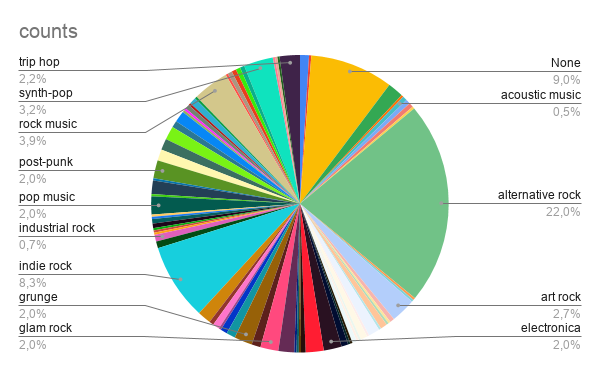
\includegraphics[width = 0.75\textwidth]{Imagenes/Bitmap/estudioGeneros.png}
	\caption{Gráfico resultado del estudio de géneros}
	\label{fig:sampleImage}
\end{figure}

En total hemos obtenido 81 géneros distintos para las canciones, entre los que destacan en gran principalmente subgéneros o géneros derivados del rock. El estilo más popular es \textbf{alternative rock}, el cual cuenta con un 22\% sobre el total, lo cual es una cantidad bastante alta en comparación con el resto. Le siguen \textbf{indie rock} y \textbf{rock music} con un 8,3\% y 3,9\% respectivamente.\\

Sin embargo, también encontramos otros géneros más distantes a los anteriores, como por ejemplo \textbf{rhythm \& blues}, \textbf{soul}, \textbf{reggae}, \textbf{jazz} o \textbf{house music}. Todos estos son estilos dispares entres sí, lo que nos da la posibilidad de ver cómo de potentes pueden ser las relaciones y explicaciones que hemos obtenido y probar nuestro sistema para ver si es capaz de relacionar canciones muy diferentes o incluso opuestas.\\

\section{Arquitectura de la aplicación}

Como punto inicial hemos utilizado varios scripts que nos ayudaron a organizar y manejar mucho mejor los datos iniciales que nos fueron proporcionados, como por ejemplo el script de limpieza y organización del dataset que, como ya hemos explicado antes, elimina cualquier tipo de valor nulo y lo ordena por popularidad, o el script de parseo, que nos permite acercarnos más a la sintaxis gramatical de Wikidata.\\

Como punto troncal, hemos desarrollado una librería que nos permite trabajar con la API de Wikidata. Hace uso de SparQL Library, la cual nos permite hacer uso del lenguaje SPARQL y hacer todo tipo de consultas a un punto. Esta librería se encarga de crear un punto de conexión a la API de Wikidata y de crear y ejecutar queries de consulta u obtención de datos hacia ese punto, el cual debe permitir el intercambio de datos en formato RDF. Además nos proporciona un objeto respuesta, el cual puede devolverse en distintos formatos.\\

La clase principal del modelo de la aplicación es getInfoSong. Esta clase hace uso de una instancia de la librería SPARQL e inicia una cadena de métodos los cuales obtienen información de distintos ámbitos de una canción proporcionada como entrada.\\

La clase Properties se encarga de establecer y configurar todas las propiedades que se van a estudiar sobre cada canción. Al crear una instancia de la clase, importa una serie de diccionarios que son almacenados. Cabe destacar que estos diccionarios son inicialmente estáticos ya que en un principio cuentan con las propiedades que hemos estudiado y probado aunque tienen la posibilidad de expandirse añadiendo nuevas propiedades, siempre que respeten la sintaxis de Wikidata. \\

Por último tenemos el módulo dataOperations, el cual es utilizado a modo auxiliar para poder convertir y hacer operaciones con los distintos dataFrames de información que se van creando continuamente al hacer un estudio de una canción.\\


\begin{figure}[h!]
	\centering
	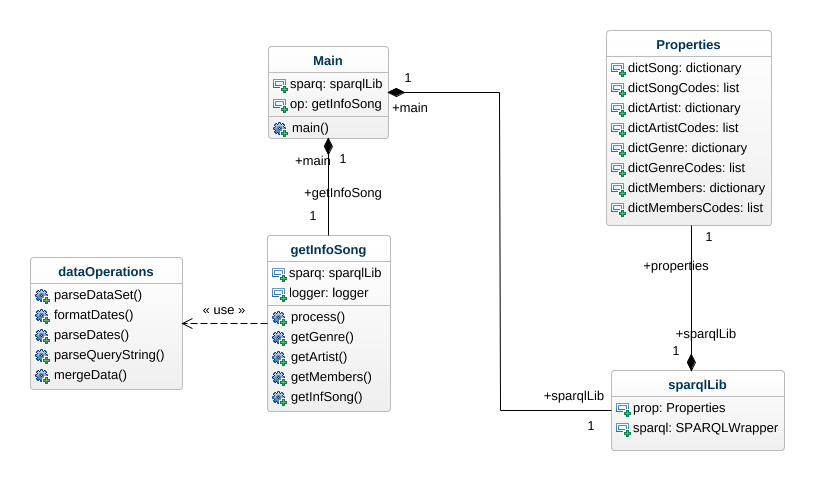
\includegraphics[width = 0.9\textwidth]{Imagenes/Bitmap/class-diagram.png}
	\caption{Diagrama de clases sobre el modelo de datos}
	\label{fig:sampleImage}
\end{figure}


